\section{Introduction}

The goal of this paper is to examine metadata from medical-related smart home devices to evaluate the vulnerabilities of Internet of Things (IoT) systems. Recent research into the security of IoT systems has revealed significant vulnerabilities that adversaries with passive network capabilities could exploit. Even when data transmitted from smart devices to home routers is encrypted, they can scrutinize metadata to obtain second order information about a user. As IoT systems expand from the home into enterprise and specialized fields, the importance of confidentiality and integrity increases. One of the most sensitive applications of IoT systems is the medical field, where patient data is extremely valuable information and needs to be closely kept in accordance with the Health Insurance Portability and Accountability Act of 1996 (HIPAA) to protect patient privacy. However, many recent innovations in medical smart home devices enable users to track their personal health using smartphones, but have the potential to leak sensitive heath information. Because of the heightened consequences of adversarial behavior in the medical field, this research focuses specifically on metadata generated from smart medical IoT devices.

\subsection{IoT Devices Studied}
The data and metadata for this project was generated from a suite of medical IoT devices currently sold on the market, including the Withings Smart Blood Pressure Monitor, Withings Smart Scale, iHealth Smart Gluco-Monitoring System, iHealth Ease Wireless Blood Pressure Monitor, and 1byOne Digital Smart Wireless Scale. These Wi-Fi or Bluetooth enabled devices are connected to a router access point or directly to a smartphone, which in turn is connected to the access point. In order to intercept traffic from the IoT devices, we configured a Raspberry Pi to serve as an access point and subsequently analyzed the traffic by classifying the streams by device, protocol, and encryption. 

\subsection{Protecting digital health information}
Though the smart medical devices we examined are intended for consumer home use, similar mIoT devices are increasingly being deployed in hospital environments and medical facilities to leverage systematic data collection and easily integrate readings and measurements into electronic health records. In these realms, mIoT devices are covered by the Security and Privacy rules of the HIPAA, which dictates core standards to protect sensitive patient information. According to a summary provided by the U.S. Department of Health and Human Services, the Security Rule Requires covered entities to maintain and appropriate administrative, technical, and physical safeguards for protecting electronic patient health information (e-PHI).$^6$ Specifically, covered entities must:

\begin{enumerate}
  \item Ensure the confidentiality, integrity, and availability of all e-PHI they create, receive, maintain, or transmit;
  \item Identify and protect against reasonably anticipated threats to the security or integrity of the information;
  \item Protect against reasonably anticipated, impermissible uses or disclosures; and
  \item Ensure compliance by their workforce. 
\end{enumerate}

Additionally, the Privacy Rule protects all individually identifiable health information held or transmitted by a covered entity or its business associate, in any form or media, whether electronic, paper or oral.$^7$ The Privacy Rule calls this information protected health information (PHI). Individually identifiable health information is information, including demographic data, that relates to:

\begin{enumerate}
  \item the individual's past, present or future physical or mental health or condition,
  \item the provision of health care to the individual, or
  \item the past, present, or future payment for the provision of health care to the individual.
\end{enumerate}

Individually identifiable health information includes many common identifiers (e.g., name, address, birth date, Social Security Number).

This paper examines whether in the course of regular behavior, smart medical devices properly protect all individually identifiable health information as dictated by HIPAA. While the name of the user or patient may be protected, network observers and adversaries can see traffic being generated from each IP address. In an age where users are inseparable from their phones, an IP address is just as much a personal identifier as a social security number. By examining network traffic from an access point, it is possible to isolate traffic originating from a fixed set of IP addresses and subsequently mine the associated metadata for sensitive medical information. 


\section{Related Work}

According to Dimiter V. Dimitrov's paper ``Medical Internet of Things and Big Data in Healthcare'' ~\cite{dimitrovIoT}, ``The Internet of Things (IoT) is a network of physical devices and other items, embedded with electronics, software, sensors, and network connectivity, which enables these objects to collect and exchange data.''$^2$ The proliferation of the Medical Internet of Things (mIoT) represents a revolution in digital healthcare because it will enable doctors and hospital systems to streamline workflows, increase productivity, and provide higher data-backed quality of care. Dimitrov highlights numerous challenges for mIoT, including 5 key capabilities that leading platforms must enable: (1) Simple connectivity, (2) Easy device management, (3) Information ingestion, (4) Informative analytics, and (5) reduced risk. Of these challenges, we attempt to improve device management and informative analytics by creating a feature of the IoT Inspector that will analyze real-time traffic flows from connected smart medical devices and inform the user of any potential privacy vulnerabilities should a device be leaking sensitive metadata. Specifically, Dimitrov specifies a need for an ``intuitive dashboard [that] makes it all easy to understand.'' We present such a dashboard in this paper, enabling average users to visualize the status of their connected devices and monitor potentially private information their devices may be transmitting without encryption. 

Although there are multiple papers that present approaches to inferring user behavior from home network traffic, most of the literature uses data collected from generic home utility devices, not medical IoT devices. For example, in ``Is Anybody Home? Inferring Activity From Start Home Network Traffic'' ~\cite{coposIoT}, Copos, Levitt et al present a scheme to infer when a home is occupied based on network traffic from a thremostat. Traffic is collected using a netbook device and then algorithms are applied to parse the packet capture files and log characteristics of the connections observed. In ``Protecting your Daily In-Home Activity Information from a Wireless Snooping Attack'' \cite{srinivasan2008fats}, Srinivasan et al present a new privacy leak in residential wireless ubiquitous computing systems, the Fingerprint and Timing-based Snooping (FATS) attack. This attack allows adversaries to observer private activities in the home such as cooking, showering, toileting, and sleeping by snooping on the wireless transmissions of sensors in a home and leveraging tiered inference algorithms.

Similarly, Apthorpe et al ~\cite{apthorpeIoT} observed that with the increasing prevalence of always-on IoT devices, writing, ``Passive network observers, such as Internet service providers, could potentially analyze IoT network traffic to infer sensitive details about users.'' By analyzing metadata from four smart home devices (a Sense sleep monitor, a Nest Cam Indoor security camera, a WeMo switch, and an Amazon Echo), Apthorpe measured the correlation between traffic rates and user interaction. He showed that even when IoT traffic is encrypted, second order information such as device activity spikes reveal potentially sensitive user information that third parties and adversaries would find valuable. These concerns are compounded when the nature of the information is personal medical data instead of consumer behavior. Particularly because of the repetitive nature of medical tests, clearly defined patterns of user activity, such as daily blood sugar or blood pressure readings, reveal common medical conditions just from metadata alone. 

Apthorpe introduces a three-step strategy that a passive network observer could use ``to identify devices in a smart home and infer user behavior.'' First, an adversary must separate the device traffic into packet streams. Second, an adversary must label streams by type of device by performing reverse DNS lookups to ``pair service IP's with device identifying domain names.'' Only once each device's traffic has been isolated, will an adversary be able to examine a device's traffic rate to infer user behavior of the device. 

In the process of examining a device's traffic, the most obvious determinant of confidentiality is encryption. Packets of data sent in the clear can be trivially intercepted by adversaries and network observers. Even if plaintext data is compressed, it is still trivial to recover the original content by recovering the compressed message and attempting decompression using a limited number of widely used compression algorithms, such as bzip. In either scenario (plaintext or compressed), an adversary is privy to first order information. For example, if a blood sugar monitor calculates the blood sugar level from an inserted test strip and transmits the results upon completion to a paired phone or access point, then a network observer can learn the actual test results in addition to the frequency with which a particular user measures his blood sugar. Transmitting application data in the clear is a severe (and seemingly obvious) design flaw, and yet it is prevalent among IoT device manufacturers. 

Even when device traffic is encrypted, as in the case of the TLS or SSL protocols, adversaries can still learn a lot from transmitted metadata. However, due to the dense nature of packet data, it is not trivial to classify traffic as encrypted or plaintext. In ``Detecting encrypted traffic: a machine learning approach'' ~\cite{chaMachineLearning}, Seunghun Cha et al. write, ``to identify encrypted traffic, the most widely used techniques are pattern matching in packet payloads and entropy analysis. Entropy-based classification is the most common method to distinguish encrypted parts from plaintexts.'' Cha outlines a four-step methodology to determining encrypted versus unencrypted traffic:

\begin{enumerate}
  \item Separate each packet's header (non-encrypted) from its payload (potentially encrypted)
  \item Analyze randomness of payload using multiple tests, including Shannon Entropy, Chi-square, and arithmetic mean
  \item Use a training subset from plaintext protocols (HTTP, FTP, Telnet) and encrypted protocols (SSH, TLS) to determine a threshold entropy, above which indicates encrypted traffic
\end{enumerate}

We employ this approach as a baseline methodology for classifying traffic. A related problem is distinguishing encrypted traffic from compressed plaintext traffic, which is more difficult since compressed and encrypted traffic exhibit high orders of entropy. In this paper, we will restrict our focus to distinguishing plaintext traffic from encrypted traffic.  

\section{Implementation}

\subsection{Approach}

To examine metadata from a suite of mIoT devices, we divided the research into three main phases: 

\begin{enumerate}
  \item Data collection
  \item Deep packet inspection
  \item Representation through a user interface
\end{enumerate}

\subsection{Data Collection}

The first step in the data collection phase was to create an isolated test environment where we could connect various mIoT devices to a network and capture live traffic. Creating an isolated test environment was necessary because it enabled us to easily separate traffic by device and filter out extraneous traffic on the network. To do this, we configured a Raspberry Pi to serve as a local access point (AP) or router, to which we would be able to connect our devices. Once the Raspberry Pi was running as a Wi-Fi router, we devised a systematic approach to collecting data. We chose four mIoT devices to inspect:

\begin{enumerate}
  \item Withings Wireless Blood Pressure Monitor
  \item Withings Body Composition Wi-Fi Scale
  \item 1byOne Digital Smart Wireless Body Fat Scale
  \item iHealth Ease Wireless Blood Pressure Monitor
\end{enumerate}

\begin{figure}
  \caption{Diagram of the data collection environment and data flow}
  \centering
    \fbox{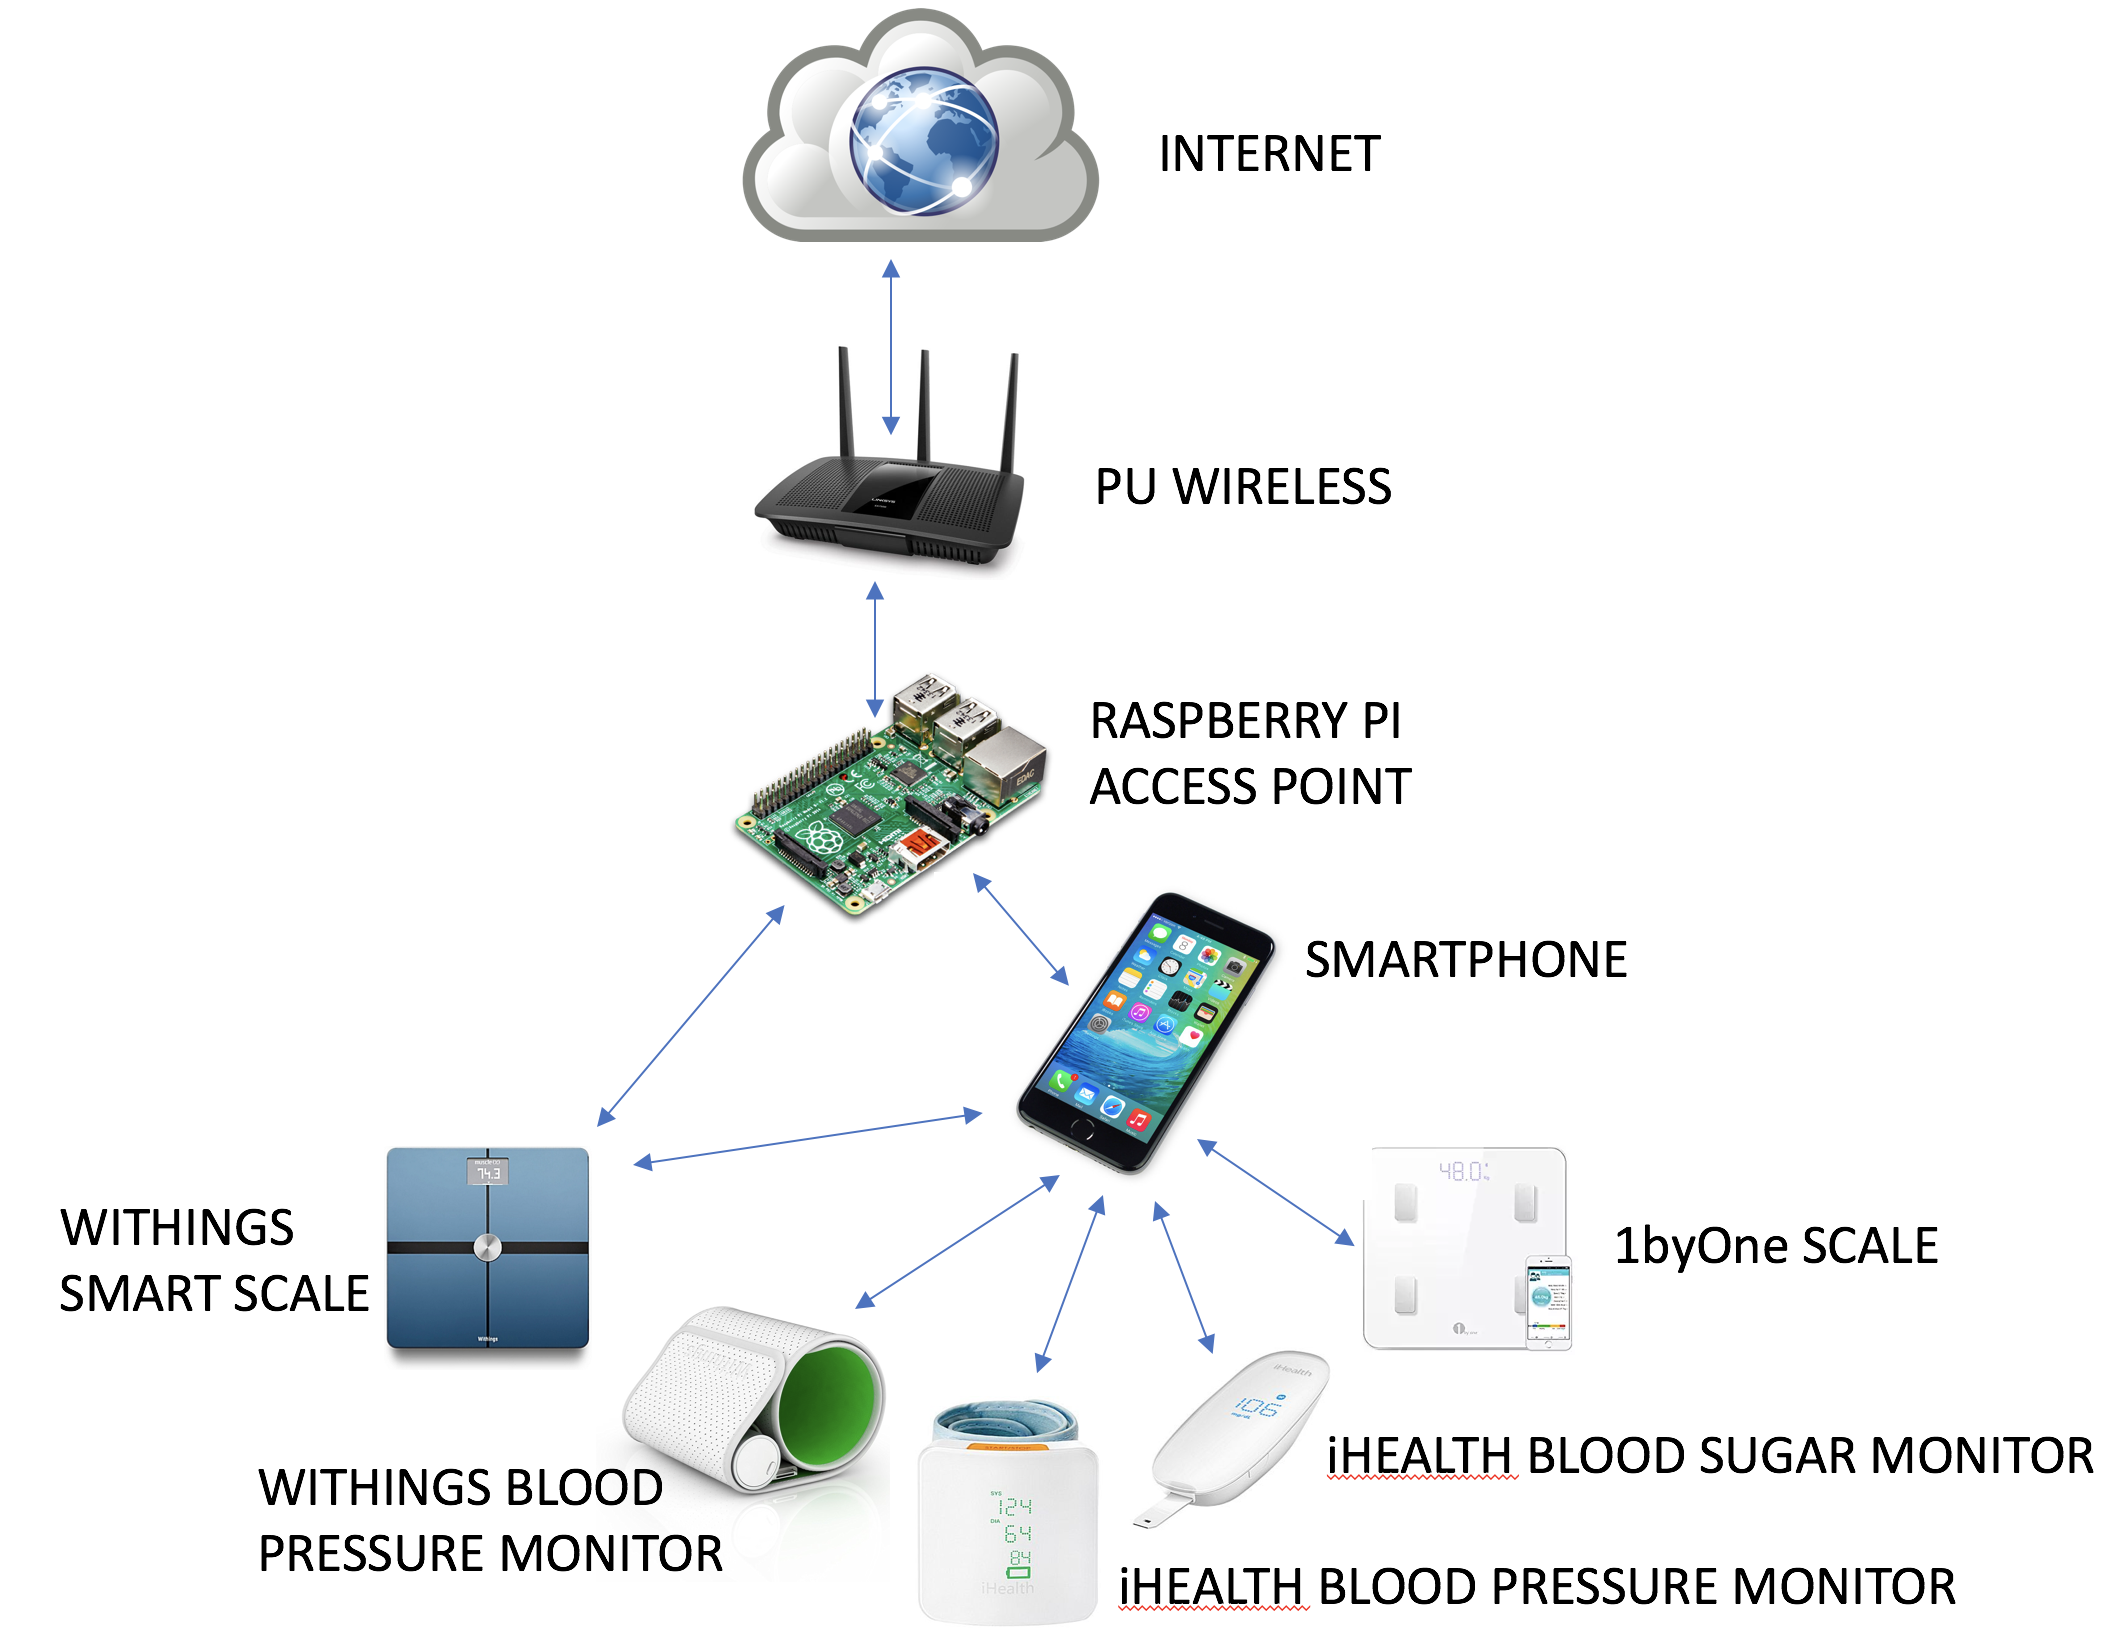
\includegraphics[scale=0.2]{network}}
\end{figure}

These devices are different from those analyzed in studies such as Apthorpe et al \cite{apthorpeIoT} because they are short-lived (i.e. only transmit data when in use for measuring blood pressure, weight, blood sugar, etc.). This provides intuitive frequency metadata and enables passive network observers to easily determine when a patient is using the device and how often. On the other hand, long-lived devices such as Amazon Echo or Nest are constantly transmitting data, though the number of packets sent increases substantially when the device is being actively used. We purposefully chose two smart scales and two blood pressure monitors so that we could compare the way in which different device manufacturers transmit application data and determine which company had better security or privacy practices, if any. 

In order to capture transmitted packets of data from the devices to the Pi, we used Wireshark to capture the Ethernet traffic being sent to the access point. We captured streams of data from each IoT device and saved it in the form of a PCAP file, which could be saved for offline analysis. When generating the dataset, we captured as many use cases of each device as possible, including user registration and sign-up, downloading patches and updates, vitals measurements, and health analytics. It is important not to ignore the use cases beyond general vitals measurement, because some of the most valuable information obtainable by an adversary would be a patch because it could reveal information about the way the embedded system in the device is designed. 

\subsection{Deep Packet Inspection}

The second phase in the project was deep packet inspection, in which we analyzed captured data streams from the suite of IoT devices for revealing metadata or unencrypted packets containing sensitive user information. We started by separating the stream of data by protocol, focusing mainly on HTTP and TCP packets and ignoring packets sent with SSL or TLS, as those are encrypted. Next we separated the payload, which contains application data, from the header of each packet for further analysis. 

The next step was to classify each incoming packet as either plaintext or encrypted. We experimented with three different schemes for this classification: naive ASCII approach, Shannon entropy test, and chi squared test. The latter two are approaches tested by Cha and Kim.~\cite{chaMachineLearning}

\subsection{Naive ASCII approach}
The first approach used to determine whether a packet was plaintext or encrypted was the naive ASCII approach. If all the characters in the payload are contained within the 128 character ASCII set, we anticipated that a packet would be unencrypted, since encrypted packets would need to contain characters from the extended ASCII set. While the naive ASCII approach does weed out encrypted packets, it does not identify all unencrypted packets, many of which contain characters from the extended ASCII set in addition to the printable characters. 

\subsection{Shannon Entropy Test}
The next approach used determine whether or not a packet was encrypted was the Shannon Entropy Test. This test calculates the entropy of each payload string, which is a quantitative measure of the variability in the frequency of the different possible characters. While random (or in this case, encrypted) strings have very high entropy, unencrypted plaintext and English strings exhibit fairly low entropy. This is because most characters are drawn from the limited set of printable characters and in English, many letters are much more likely to appear than others. For example, the letter e appears roughly 12.5\% of the time, while the letter $j$ appears less than 0.2\% of the time. To calculate the Shannon Entropy of a string, let $X$ be a random variable that takes on possible values $x_1$, $x_2$, ..., $x_n$. $p(x_i)$ is the probability that $X = x_i$:

$$H(X) = - \sum_{i = 1}^{n} p(x_i) log p(x_i)$$

A packet's payload is presumed to be unencrypted if its Shannon entropy value is lower than a threshold perameter, which can be tuned between 4 - 8. 

\subsection{Chi Squared Test}
Lastly, the Chi Squared test compares the frequency of each character with its expected value from a uniform distribution. The value $x^2$ is calculated according to the formula:

$$X^2 = \sum_{i=1}^{n} \frac{(o_i-e_i)^2}{e_i}$$

The more a set of frequencies deviates from its expected values, the higher the value of $x^2$, and if the observed frequencies equal the expected frequencies then $x^2$ is 0. Therefore, English plaintext is expected to have a much higher deviation of character frequencies from the expected frequency (a uniformly random distribution). By setting the threshold value $x^2 = 1000$, we were able to effectively weed out the unencrypted payloads from those that were encrypted. 

\subsection{Method Comparison}
In order to determine which of the three methods (naive ASCII, Shannon Entropy, or Chi Squared) yielded the most accurate classification of unencrypted packets, we ran a comparative analysis with five PCAP files with over 75,000 packets. Out of the three methods, the naive ascii approach was the most selective. It had a 0 percent false positive rate, but missed nearly all of the unencrypted packets, because many of the payloads contained some number extended ASCII characters. 

In contrast, the Shannon Entropy approach cast a much wider net, tagging a much larger share of packets as being unencrypted, though this approach suffered from a high false positive rate. Lowering the threshold entropy value did not significantly increase the accuracy of the approach, as fewer true unencrypted packets were identified as the threshold entropy value decreased. 

We found the most accurate encryption classification approach to be the Chi Square test, due to its low false positive rate and identification of non-random string patterns within the packet payloads we tested. The Chi Square test exhibited a false positive rate of approximately 3.5 percent, while still identifying nearly all the other unencrypted payloads as the naive ascii and Shannon entropy approaches.


\begin{figure}
  \caption{Comparison of plaintext detection approaches}
  \begin{center}
    \begin{tabular}{||c c c||} 
    \hline
    Approach & False Positve Rate & \% packets plaintext\\ [0.5ex] 
    \hline\hline
    Naive ASCII & $0.0$ & $0.005$ \\ 
    \hline
    Shannon Entropy &  $0.74$ & $0.162$ \\
    \hline
    Chi Square & $0.03$ & $0.049$ \\
    \hline
    \end{tabular}
  \end{center}
\end{figure}

\subsection{Dictionary Analysis}
Once we were able to identify plaintext packets, we identified potentially sensitive personal medical/identifying information by searching each string in the plaintext payload in several dictionaries. We used three dictionaries: a list of the 100 most common medical terms/conditions, a list of the most popular first male and female names, and a list of the most common personal identifying information (i.e. passport number, license, name, address, etc.). 

\subsection{Representing the Results}

The final goal of our research effort was to design a hub for consumers to connect their smart home devices and easily monitor potential confidentiality breaches during regular device usage through a user interface. The hub, programmed on a Raspberry Pi, acted as a Wi-Fi and Bluetooth access point. Since all device traffic flows through the hub, we were able to capture and analyze the transmitted data from each device and display potential vulnerabilities on a dashboard running on the Raspberry Pi. 

Because consumers currently have no visibility into the types of traffic and information their devices are transmitting across the internet, the objective was to design a user-friendly interface that would alert each user of potentially confidential or private information that was discovered using this paper's deep packet inspection approach. The dashboard simply displayed each connected device, followed by a list of personally identifiable information or medical terms discovered in the course of deep packet inspection. 

\section{Results}

After conducting deep packet analysis on each of the IoT devices, we found a very large variability in the methods each device used to send application data through the network when registering users, sending patches and updates, measuring vitals, or retrieving health analytics. All of the devices used encryption and protocols such as TLS or SSH to send sensitive first order information, such as the user's actual weight or blood sugar levels. However, there were various degrees of leaking second order information and metadata, scraped from sources such as HTTP GET requests, packet header information, and device conversation IP tables. Of the devices that we captured traffic for, the most secure implementation was the 1byOne Digital Smart Wireless Body Fat Scale. This device not only used encrypted protocols to deliver application data, but also masked names of packet destinations, unlike the Withings devices. 

\subsection{Blood pressure monitor leaks information}
The Withings Blood Pressure Monitor, out of the four devices monitored, exhibited the most number of vulnerabilities when it comes to revealing sensitive user information during data transmission. We were able to capture enough sensitive second order data and metadata from a stream of traffic from the device in the course of typical usage to determine that the user of the device was measuring his or her blood pressure, and how frequently as well. 

First of all, it is very easy for a network observer to detect that a Withings IoT device is in use, because the information sections of all queries and responses to the Withings servers are titled with the brand of the device in the URL. This would make it exceptionally easy for a network observer to track all traffic originating from IP addresses querying an address such as static.withings.com. Because of the limited capabilities of medical IoT devices, as opposed to devices such as Amazon Echo, which can reach any endpoint on the Internet, there is a limited number of endpoints that are queried from each device, making device identification by a network observer trivial.

Even more concerning, we observed that one of the signature characteristics of the Withings Blood Pressure Monitor's traffic pattern was the fact that each digital reading concluded with a GET request for a stock photo of a person using the Withings Blood Pressure Monitor (Figure 3). This GET request is certainly a cause for concern, as any adversary monitoring the traffic would be able to immediately determine when a user has finished measuring his or her blood pressure. This GET request was sent completely in the clear, and furthermore, it is not even displayed on the user interface of the app to the user of the device. It appears that there is no purpose of sending this image upon the success of each blood pressure reading, except inadvertently notifying network observers that the Withings Blood Pressure Monitor is in use. 

\begin{figure}
  \caption{Withings Blood Pressure Monitor sends image in the clear}
  \centering
    \fbox{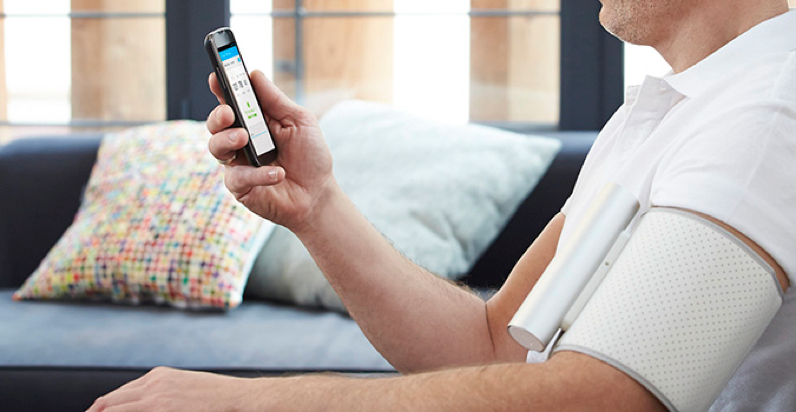
\includegraphics[scale=0.5]{bloodpressure}}
\end{figure}

\begin{figure}
  \caption{Captured HTTP Packet reveals nature of device/user behavior}
  \centering
    \fbox{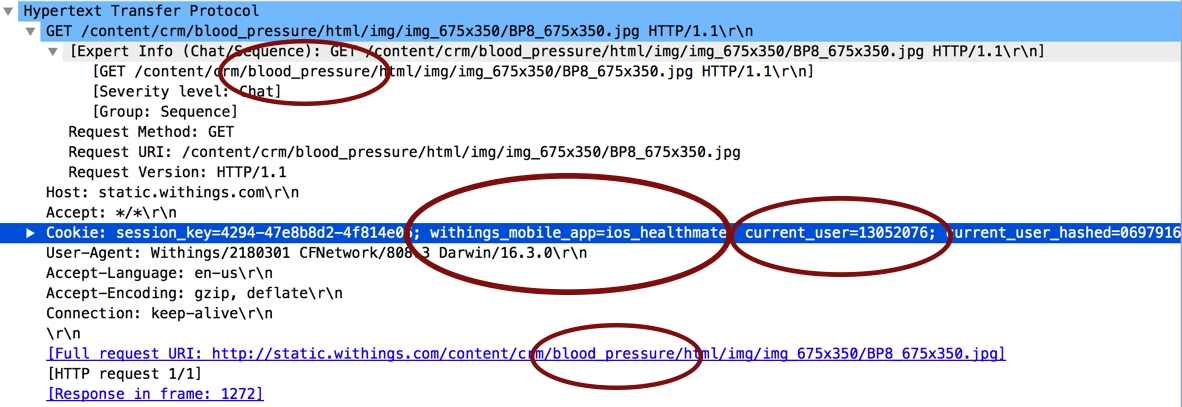
\includegraphics[scale=0.4]{bloodpacket}}
\end{figure}

Figure 4 highlights the example of one packet alone, which revealed four sources of valuable information about the device. The plaintext string ``blood\textunderscore pressure'' appears twice, along with the string ``withings\textunderscore mobile\textunderscore app=ios\textunderscore healthmate''. Lastly, the ``current\textunderscore user'' field, while not directly disclosing the name of user, is potentially a unique identifier that associates that user with the subsequent blood pressure data. By monitoring this traffic for a period of time with many users, it would be trivial to match each packet of transmitted application data to the associated user. 

\subsection{Smart scale encrypts user data}
In sharp contrast to the Withings Blood Pressure Monitor, the 1byOne Smart Scale was actually very secure. After pairing the scale with a smartphone and connecting it to the test network to capture the transmitted packets, we found that the Smart Scale actually used TLSv1.2 on port 443 to send encrypted application data. Additionally, even though the scale only transmited data when it was being used to measure weight, the traffic was difficult to detect without knowing the exact source IP address, since the packets are not labeled with revealing information about the nature of the device, and the destination addresses are not readable URLs such as the case of the Withings Blood Pressure Monitor. 

Therefore, when we ran the deep packet analysis of the traffic of the 1byOne Smart Scale, it was not possible to compile information about the user's behavior in the same way as with the blood pressure monitor. 


\section{Discussion}

The sheer diversity of devices, protocols, and lack of standardization between device manufacturers makes it very difficult to detect all vulnerabilities, or to even identify all of the devices that are connected to a network.

This research suggests that medical IoT device manufacturers are not necessarily aligned with policies including the Privacy and Security rules of HIPAA, and they may inadvertently reveal sensitive data and metadata about a user's behavior and medical condition. For example, the Privacy rule dictates that manufacturers and medical professionals protect personally identifying information such as the individual's past, present or future physical or mental health or condition. Though we found no instances of full names or biologically identifiable information being leaked, in the digital age, policy makers and manufacturers should recognize the increasingly identifiable nature of IP addresses. With users carrying smartphones in their pockets 24 hours a day, completing transactions, querying the Internet, and communicating with friends, an IP address is perhaps more individually identifiable than a social security number.

Lastly, this research underscores the lack of awareness among the general public when it comes to the confidentiality and integrity of their personal data. As technology becomes increasingly capable and complex, it will only become more difficult for users of connected devices to comprehend what sort of data can be extracted from their digital footprint, even if the devices they are using encrypt first order information. Tools like the user interface presented in this paper are in the public interest to increase the visibility of device vulnerabilities, awareness of personal confidentiality weaknesses, and accountability among device manufacturers.


\section{Conclusion}

These results reveal multiple known vulnerabilities within IoT devices, but there are heightened implications due to the sensitive nature of the medical metadata being disclosed. Particularly if used by healthcare professionals to measure patient vital signs/data over time, these medical IoT devices need to be more carefully examined by regulators and physician networks to increase the awareness of this information leakage before they are implemented on a wider scale. 

\appendix

\section*{Acknowledgements}
Thanks to Nick Feamster, Noah Apthorpe, Dillon Reisman, Rohan Doshi, and Gudrun Jonsdottir for their thoughts and contributions to the discussions that focused this work. 
